\documentclass[10pt]{article}
\usepackage[preprint]{tmlr}
%%%%% NEW MATH DEFINITIONS %%%%%

\usepackage{amsmath,amsfonts,bm}

% Mark sections of captions for referring to divisions of figures
\newcommand{\figleft}{{\em (Left)}}
\newcommand{\figcenter}{{\em (Center)}}
\newcommand{\figright}{{\em (Right)}}
\newcommand{\figtop}{{\em (Top)}}
\newcommand{\figbottom}{{\em (Bottom)}}
\newcommand{\captiona}{{\em (a)}}
\newcommand{\captionb}{{\em (b)}}
\newcommand{\captionc}{{\em (c)}}
\newcommand{\captiond}{{\em (d)}}

% Highlight a newly defined term
\newcommand{\newterm}[1]{{\bf #1}}


% Figure reference, lower-case.
\def\figref#1{figure~\ref{#1}}
% Figure reference, capital. For start of sentence
\def\Figref#1{Figure~\ref{#1}}
\def\twofigref#1#2{figures \ref{#1} and \ref{#2}}
\def\quadfigref#1#2#3#4{figures \ref{#1}, \ref{#2}, \ref{#3} and \ref{#4}}
% Section reference, lower-case.
\def\secref#1{section~\ref{#1}}
% Section reference, capital.
\def\Secref#1{Section~\ref{#1}}
% Reference to two sections.
\def\twosecrefs#1#2{sections \ref{#1} and \ref{#2}}
% Reference to three sections.
\def\secrefs#1#2#3{sections \ref{#1}, \ref{#2} and \ref{#3}}
% Reference to an equation, lower-case.
\def\eqref#1{equation~\ref{#1}}
% Reference to an equation, upper case
\def\Eqref#1{Equation~\ref{#1}}
% A raw reference to an equation---avoid using if possible
\def\plaineqref#1{\ref{#1}}
% Reference to a chapter, lower-case.
\def\chapref#1{chapter~\ref{#1}}
% Reference to an equation, upper case.
\def\Chapref#1{Chapter~\ref{#1}}
% Reference to a range of chapters
\def\rangechapref#1#2{chapters\ref{#1}--\ref{#2}}
% Reference to an algorithm, lower-case.
\def\algref#1{algorithm~\ref{#1}}
% Reference to an algorithm, upper case.
\def\Algref#1{Algorithm~\ref{#1}}
\def\twoalgref#1#2{algorithms \ref{#1} and \ref{#2}}
\def\Twoalgref#1#2{Algorithms \ref{#1} and \ref{#2}}
% Reference to a part, lower case
\def\partref#1{part~\ref{#1}}
% Reference to a part, upper case
\def\Partref#1{Part~\ref{#1}}
\def\twopartref#1#2{parts \ref{#1} and \ref{#2}}

\def\ceil#1{\lceil #1 \rceil}
\def\floor#1{\lfloor #1 \rfloor}
\def\1{\bm{1}}
\newcommand{\train}{\mathcal{D}}
\newcommand{\valid}{\mathcal{D_{\mathrm{valid}}}}
\newcommand{\test}{\mathcal{D_{\mathrm{test}}}}

\def\eps{{\epsilon}}


% Random variables
\def\reta{{\textnormal{$\eta$}}}
\def\ra{{\textnormal{a}}}
\def\rb{{\textnormal{b}}}
\def\rc{{\textnormal{c}}}
\def\rd{{\textnormal{d}}}
\def\re{{\textnormal{e}}}
\def\rf{{\textnormal{f}}}
\def\rg{{\textnormal{g}}}
\def\rh{{\textnormal{h}}}
\def\ri{{\textnormal{i}}}
\def\rj{{\textnormal{j}}}
\def\rk{{\textnormal{k}}}
\def\rl{{\textnormal{l}}}
% rm is already a command, just don't name any random variables m
\def\rn{{\textnormal{n}}}
\def\ro{{\textnormal{o}}}
\def\rp{{\textnormal{p}}}
\def\rq{{\textnormal{q}}}
\def\rr{{\textnormal{r}}}
\def\rs{{\textnormal{s}}}
\def\rt{{\textnormal{t}}}
\def\ru{{\textnormal{u}}}
\def\rv{{\textnormal{v}}}
\def\rw{{\textnormal{w}}}
\def\rx{{\textnormal{x}}}
\def\ry{{\textnormal{y}}}
\def\rz{{\textnormal{z}}}

% Random vectors
\def\rvepsilon{{\mathbf{\epsilon}}}
\def\rvtheta{{\mathbf{\theta}}}
\def\rva{{\mathbf{a}}}
\def\rvb{{\mathbf{b}}}
\def\rvc{{\mathbf{c}}}
\def\rvd{{\mathbf{d}}}
\def\rve{{\mathbf{e}}}
\def\rvf{{\mathbf{f}}}
\def\rvg{{\mathbf{g}}}
\def\rvh{{\mathbf{h}}}
\def\rvu{{\mathbf{i}}}
\def\rvj{{\mathbf{j}}}
\def\rvk{{\mathbf{k}}}
\def\rvl{{\mathbf{l}}}
\def\rvm{{\mathbf{m}}}
\def\rvn{{\mathbf{n}}}
\def\rvo{{\mathbf{o}}}
\def\rvp{{\mathbf{p}}}
\def\rvq{{\mathbf{q}}}
\def\rvr{{\mathbf{r}}}
\def\rvs{{\mathbf{s}}}
\def\rvt{{\mathbf{t}}}
\def\rvu{{\mathbf{u}}}
\def\rvv{{\mathbf{v}}}
\def\rvw{{\mathbf{w}}}
\def\rvx{{\mathbf{x}}}
\def\rvy{{\mathbf{y}}}
\def\rvz{{\mathbf{z}}}

% Elements of random vectors
\def\erva{{\textnormal{a}}}
\def\ervb{{\textnormal{b}}}
\def\ervc{{\textnormal{c}}}
\def\ervd{{\textnormal{d}}}
\def\erve{{\textnormal{e}}}
\def\ervf{{\textnormal{f}}}
\def\ervg{{\textnormal{g}}}
\def\ervh{{\textnormal{h}}}
\def\ervi{{\textnormal{i}}}
\def\ervj{{\textnormal{j}}}
\def\ervk{{\textnormal{k}}}
\def\ervl{{\textnormal{l}}}
\def\ervm{{\textnormal{m}}}
\def\ervn{{\textnormal{n}}}
\def\ervo{{\textnormal{o}}}
\def\ervp{{\textnormal{p}}}
\def\ervq{{\textnormal{q}}}
\def\ervr{{\textnormal{r}}}
\def\ervs{{\textnormal{s}}}
\def\ervt{{\textnormal{t}}}
\def\ervu{{\textnormal{u}}}
\def\ervv{{\textnormal{v}}}
\def\ervw{{\textnormal{w}}}
\def\ervx{{\textnormal{x}}}
\def\ervy{{\textnormal{y}}}
\def\ervz{{\textnormal{z}}}

% Random matrices
\def\rmA{{\mathbf{A}}}
\def\rmB{{\mathbf{B}}}
\def\rmC{{\mathbf{C}}}
\def\rmD{{\mathbf{D}}}
\def\rmE{{\mathbf{E}}}
\def\rmF{{\mathbf{F}}}
\def\rmG{{\mathbf{G}}}
\def\rmH{{\mathbf{H}}}
\def\rmI{{\mathbf{I}}}
\def\rmJ{{\mathbf{J}}}
\def\rmK{{\mathbf{K}}}
\def\rmL{{\mathbf{L}}}
\def\rmM{{\mathbf{M}}}
\def\rmN{{\mathbf{N}}}
\def\rmO{{\mathbf{O}}}
\def\rmP{{\mathbf{P}}}
\def\rmQ{{\mathbf{Q}}}
\def\rmR{{\mathbf{R}}}
\def\rmS{{\mathbf{S}}}
\def\rmT{{\mathbf{T}}}
\def\rmU{{\mathbf{U}}}
\def\rmV{{\mathbf{V}}}
\def\rmW{{\mathbf{W}}}
\def\rmX{{\mathbf{X}}}
\def\rmY{{\mathbf{Y}}}
\def\rmZ{{\mathbf{Z}}}

% Elements of random matrices
\def\ermA{{\textnormal{A}}}
\def\ermB{{\textnormal{B}}}
\def\ermC{{\textnormal{C}}}
\def\ermD{{\textnormal{D}}}
\def\ermE{{\textnormal{E}}}
\def\ermF{{\textnormal{F}}}
\def\ermG{{\textnormal{G}}}
\def\ermH{{\textnormal{H}}}
\def\ermI{{\textnormal{I}}}
\def\ermJ{{\textnormal{J}}}
\def\ermK{{\textnormal{K}}}
\def\ermL{{\textnormal{L}}}
\def\ermM{{\textnormal{M}}}
\def\ermN{{\textnormal{N}}}
\def\ermO{{\textnormal{O}}}
\def\ermP{{\textnormal{P}}}
\def\ermQ{{\textnormal{Q}}}
\def\ermR{{\textnormal{R}}}
\def\ermS{{\textnormal{S}}}
\def\ermT{{\textnormal{T}}}
\def\ermU{{\textnormal{U}}}
\def\ermV{{\textnormal{V}}}
\def\ermW{{\textnormal{W}}}
\def\ermX{{\textnormal{X}}}
\def\ermY{{\textnormal{Y}}}
\def\ermZ{{\textnormal{Z}}}

% Vectors
\def\vzero{{\bm{0}}}
\def\vone{{\bm{1}}}
\def\vmu{{\bm{\mu}}}
\def\vtheta{{\bm{\theta}}}
\def\va{{\bm{a}}}
\def\vb{{\bm{b}}}
\def\vc{{\bm{c}}}
\def\vd{{\bm{d}}}
\def\ve{{\bm{e}}}
\def\vf{{\bm{f}}}
\def\vg{{\bm{g}}}
\def\vh{{\bm{h}}}
\def\vi{{\bm{i}}}
\def\vj{{\bm{j}}}
\def\vk{{\bm{k}}}
\def\vl{{\bm{l}}}
\def\vm{{\bm{m}}}
\def\vn{{\bm{n}}}
\def\vo{{\bm{o}}}
\def\vp{{\bm{p}}}
\def\vq{{\bm{q}}}
\def\vr{{\bm{r}}}
\def\vs{{\bm{s}}}
\def\vt{{\bm{t}}}
\def\vu{{\bm{u}}}
\def\vv{{\bm{v}}}
\def\vw{{\bm{w}}}
\def\vx{{\bm{x}}}
\def\vy{{\bm{y}}}
\def\vz{{\bm{z}}}

% Elements of vectors
\def\evalpha{{\alpha}}
\def\evbeta{{\beta}}
\def\evepsilon{{\epsilon}}
\def\evlambda{{\lambda}}
\def\evomega{{\omega}}
\def\evmu{{\mu}}
\def\evpsi{{\psi}}
\def\evsigma{{\sigma}}
\def\evtheta{{\theta}}
\def\eva{{a}}
\def\evb{{b}}
\def\evc{{c}}
\def\evd{{d}}
\def\eve{{e}}
\def\evf{{f}}
\def\evg{{g}}
\def\evh{{h}}
\def\evi{{i}}
\def\evj{{j}}
\def\evk{{k}}
\def\evl{{l}}
\def\evm{{m}}
\def\evn{{n}}
\def\evo{{o}}
\def\evp{{p}}
\def\evq{{q}}
\def\evr{{r}}
\def\evs{{s}}
\def\evt{{t}}
\def\evu{{u}}
\def\evv{{v}}
\def\evw{{w}}
\def\evx{{x}}
\def\evy{{y}}
\def\evz{{z}}

% Matrix
\def\mA{{\bm{A}}}
\def\mB{{\bm{B}}}
\def\mC{{\bm{C}}}
\def\mD{{\bm{D}}}
\def\mE{{\bm{E}}}
\def\mF{{\bm{F}}}
\def\mG{{\bm{G}}}
\def\mH{{\bm{H}}}
\def\mI{{\bm{I}}}
\def\mJ{{\bm{J}}}
\def\mK{{\bm{K}}}
\def\mL{{\bm{L}}}
\def\mM{{\bm{M}}}
\def\mN{{\bm{N}}}
\def\mO{{\bm{O}}}
\def\mP{{\bm{P}}}
\def\mQ{{\bm{Q}}}
\def\mR{{\bm{R}}}
\def\mS{{\bm{S}}}
\def\mT{{\bm{T}}}
\def\mU{{\bm{U}}}
\def\mV{{\bm{V}}}
\def\mW{{\bm{W}}}
\def\mX{{\bm{X}}}
\def\mY{{\bm{Y}}}
\def\mZ{{\bm{Z}}}
\def\mBeta{{\bm{\beta}}}
\def\mPhi{{\bm{\Phi}}}
\def\mLambda{{\bm{\Lambda}}}
\def\mSigma{{\bm{\Sigma}}}

% Tensor
\DeclareMathAlphabet{\mathsfit}{\encodingdefault}{\sfdefault}{m}{sl}
\SetMathAlphabet{\mathsfit}{bold}{\encodingdefault}{\sfdefault}{bx}{n}
\newcommand{\tens}[1]{\bm{\mathsfit{#1}}}
\def\tA{{\tens{A}}}
\def\tB{{\tens{B}}}
\def\tC{{\tens{C}}}
\def\tD{{\tens{D}}}
\def\tE{{\tens{E}}}
\def\tF{{\tens{F}}}
\def\tG{{\tens{G}}}
\def\tH{{\tens{H}}}
\def\tI{{\tens{I}}}
\def\tJ{{\tens{J}}}
\def\tK{{\tens{K}}}
\def\tL{{\tens{L}}}
\def\tM{{\tens{M}}}
\def\tN{{\tens{N}}}
\def\tO{{\tens{O}}}
\def\tP{{\tens{P}}}
\def\tQ{{\tens{Q}}}
\def\tR{{\tens{R}}}
\def\tS{{\tens{S}}}
\def\tT{{\tens{T}}}
\def\tU{{\tens{U}}}
\def\tV{{\tens{V}}}
\def\tW{{\tens{W}}}
\def\tX{{\tens{X}}}
\def\tY{{\tens{Y}}}
\def\tZ{{\tens{Z}}}


% Graph
\def\gA{{\mathcal{A}}}
\def\gB{{\mathcal{B}}}
\def\gC{{\mathcal{C}}}
\def\gD{{\mathcal{D}}}
\def\gE{{\mathcal{E}}}
\def\gF{{\mathcal{F}}}
\def\gG{{\mathcal{G}}}
\def\gH{{\mathcal{H}}}
\def\gI{{\mathcal{I}}}
\def\gJ{{\mathcal{J}}}
\def\gK{{\mathcal{K}}}
\def\gL{{\mathcal{L}}}
\def\gM{{\mathcal{M}}}
\def\gN{{\mathcal{N}}}
\def\gO{{\mathcal{O}}}
\def\gP{{\mathcal{P}}}
\def\gQ{{\mathcal{Q}}}
\def\gR{{\mathcal{R}}}
\def\gS{{\mathcal{S}}}
\def\gT{{\mathcal{T}}}
\def\gU{{\mathcal{U}}}
\def\gV{{\mathcal{V}}}
\def\gW{{\mathcal{W}}}
\def\gX{{\mathcal{X}}}
\def\gY{{\mathcal{Y}}}
\def\gZ{{\mathcal{Z}}}

% Sets
\def\sA{{\mathbb{A}}}
\def\sB{{\mathbb{B}}}
\def\sC{{\mathbb{C}}}
\def\sD{{\mathbb{D}}}
% Don't use a set called E, because this would be the same as our symbol
% for expectation.
\def\sF{{\mathbb{F}}}
\def\sG{{\mathbb{G}}}
\def\sH{{\mathbb{H}}}
\def\sI{{\mathbb{I}}}
\def\sJ{{\mathbb{J}}}
\def\sK{{\mathbb{K}}}
\def\sL{{\mathbb{L}}}
\def\sM{{\mathbb{M}}}
\def\sN{{\mathbb{N}}}
\def\sO{{\mathbb{O}}}
\def\sP{{\mathbb{P}}}
\def\sQ{{\mathbb{Q}}}
\def\sR{{\mathbb{R}}}
\def\sS{{\mathbb{S}}}
\def\sT{{\mathbb{T}}}
\def\sU{{\mathbb{U}}}
\def\sV{{\mathbb{V}}}
\def\sW{{\mathbb{W}}}
\def\sX{{\mathbb{X}}}
\def\sY{{\mathbb{Y}}}
\def\sZ{{\mathbb{Z}}}

% Entries of a matrix
\def\emLambda{{\Lambda}}
\def\emA{{A}}
\def\emB{{B}}
\def\emC{{C}}
\def\emD{{D}}
\def\emE{{E}}
\def\emF{{F}}
\def\emG{{G}}
\def\emH{{H}}
\def\emI{{I}}
\def\emJ{{J}}
\def\emK{{K}}
\def\emL{{L}}
\def\emM{{M}}
\def\emN{{N}}
\def\emO{{O}}
\def\emP{{P}}
\def\emQ{{Q}}
\def\emR{{R}}
\def\emS{{S}}
\def\emT{{T}}
\def\emU{{U}}
\def\emV{{V}}
\def\emW{{W}}
\def\emX{{X}}
\def\emY{{Y}}
\def\emZ{{Z}}
\def\emSigma{{\Sigma}}

% entries of a tensor
% Same font as tensor, without \bm wrapper
\newcommand{\etens}[1]{\mathsfit{#1}}
\def\etLambda{{\etens{\Lambda}}}
\def\etA{{\etens{A}}}
\def\etB{{\etens{B}}}
\def\etC{{\etens{C}}}
\def\etD{{\etens{D}}}
\def\etE{{\etens{E}}}
\def\etF{{\etens{F}}}
\def\etG{{\etens{G}}}
\def\etH{{\etens{H}}}
\def\etI{{\etens{I}}}
\def\etJ{{\etens{J}}}
\def\etK{{\etens{K}}}
\def\etL{{\etens{L}}}
\def\etM{{\etens{M}}}
\def\etN{{\etens{N}}}
\def\etO{{\etens{O}}}
\def\etP{{\etens{P}}}
\def\etQ{{\etens{Q}}}
\def\etR{{\etens{R}}}
\def\etS{{\etens{S}}}
\def\etT{{\etens{T}}}
\def\etU{{\etens{U}}}
\def\etV{{\etens{V}}}
\def\etW{{\etens{W}}}
\def\etX{{\etens{X}}}
\def\etY{{\etens{Y}}}
\def\etZ{{\etens{Z}}}

% The true underlying data generating distribution
\newcommand{\pdata}{p_{\rm{data}}}
% The empirical distribution defined by the training set
\newcommand{\ptrain}{\hat{p}_{\rm{data}}}
\newcommand{\Ptrain}{\hat{P}_{\rm{data}}}
% The model distribution
\newcommand{\pmodel}{p_{\rm{model}}}
\newcommand{\Pmodel}{P_{\rm{model}}}
\newcommand{\ptildemodel}{\tilde{p}_{\rm{model}}}
% Stochastic autoencoder distributions
\newcommand{\pencode}{p_{\rm{encoder}}}
\newcommand{\pdecode}{p_{\rm{decoder}}}
\newcommand{\precons}{p_{\rm{reconstruct}}}

\newcommand{\laplace}{\mathrm{Laplace}} % Laplace distribution

\newcommand{\E}{\mathbb{E}}
\newcommand{\Ls}{\mathcal{L}}
\newcommand{\R}{\mathbb{R}}
\newcommand{\emp}{\tilde{p}}
\newcommand{\lr}{\alpha}
\newcommand{\reg}{\lambda}
\newcommand{\rect}{\mathrm{rectifier}}
\newcommand{\softmax}{\mathrm{softmax}}
\newcommand{\sigmoid}{\sigma}
\newcommand{\softplus}{\zeta}
\newcommand{\KL}{D_{\mathrm{KL}}}
\newcommand{\Var}{\mathrm{Var}}
\newcommand{\standarderror}{\mathrm{SE}}
\newcommand{\Cov}{\mathrm{Cov}}
% Wolfram Mathworld says $L^2$ is for function spaces and $\ell^2$ is for vectors
% But then they seem to use $L^2$ for vectors throughout the site, and so does
% wikipedia.
\newcommand{\normlzero}{L^0}
\newcommand{\normlone}{L^1}
\newcommand{\normltwo}{L^2}
\newcommand{\normlp}{L^p}
\newcommand{\normmax}{L^\infty}

\newcommand{\parents}{Pa} % See usage in notation.tex. Chosen to match Daphne's book.

\DeclareMathOperator*{\argmax}{arg\,max}
\DeclareMathOperator*{\argmin}{arg\,min}

\DeclareMathOperator{\sign}{sign}
\DeclareMathOperator{\Tr}{Tr}
\let\ab\allowbreak

\usepackage[hidelinks]{hyperref}
\usepackage{url}
\usepackage{array}
\usepackage{float}
\usepackage[font=small,labelfont=bf,labelsep=period,skip=5pt]{caption}
\usepackage{booktabs}
\usepackage{verbatim}
\usepackage{graphicx}
\usepackage{amsmath,amssymb}
\usepackage{microtype}
\usepackage{xcolor}
% generated by scripts/make_paper_assets.py
\newcommand{\Ncore}{120}
\newcommand{\Ntasks}{360}
\newcommand{\ablFewTasks}{12}
\newcommand{\ablFracAllRuns}{95\%}
\newcommand{\ablFracFewTasks}{12\%}
\newcommand{\ablFracOneRun}{85\%}
\newcommand{\ablTauAllRuns}{1.00}
\newcommand{\ablTauFewTasks}{0.86}
\newcommand{\ablTauOneRun}{0.98}
\newcommand{\covBBTenRuns}{95.1\%}
\newcommand{\covBCaTenRuns}{94.8\%}
\newcommand{\covBootRange}{92.5\%--95.1\%}
\newcommand{\covBootTenRuns}{94.8\%}
\newcommand{\covCPTenRuns}{68.3\%}
\newcommand{\covPassKMax}{94.8\%}
\newcommand{\covPassKMin}{90.8\%}
\newcommand{\covRunsTenRuns}{56.4\%}
\newcommand{\covTwoTenRuns}{96.4\%}
\newcommand{\covWilsonTenRuns}{68.3\%}
\newcommand{\covWilsonThreeRuns}{88.5\%}
\newcommand{\designBudget}{1200}
\newcommand{\designMaxSEgap}{3.8\%}
\newcommand{\designPowerOne}{68.7\%}
\newcommand{\designPowerTen}{47.9\%}
\newcommand{\designPowerTwenty}{36.7\%}
\newcommand{\designSEratio}{1.60}
\newcommand{\rankCovMax}{99.9\%}
\newcommand{\rankCovMin}{98.6\%}
\newcommand{\realBestModel}{qwen2.5-7b}
\newcommand{\realBestPassOne}{63.7\%}
\newcommand{\realBestPassTen}{40.8\%}
\newcommand{\realBestPassThree}{52.9\%}
\newcommand{\realBestScore}{63.7\%}
\newcommand{\realClosestA}{llama3.2-3b}
\newcommand{\realClosestB}{qwen2.5-3b}
\newcommand{\realClosestDiff}{1.7}
\newcommand{\realClosestP}{0.67}
\newcommand{\realFloorNoAction}{100\%}
\newcommand{\realFracSep}{95\%}
\newcommand{\realG}{0.99}
\newcommand{\realInterShare}{26\%}
\newcommand{\realMDE}{9.0}
\newcommand{\realMaxStepLimit}{42\%}
\newcommand{\realMaxStepLimitModel}{llama3.2-1b}
\newcommand{\realModelShare}{25\%}
\newcommand{\realNAttempts}{8\,400}
\newcommand{\realNFloor}{2}
\newcommand{\realNIndist}{1}
\newcommand{\realNModels}{7}
\newcommand{\realNPairs}{21}
\newcommand{\realNRuns}{10}
\newcommand{\realNTasks}{120}
\newcommand{\realOptRuns}{4}
\newcommand{\realRunShare}{34\%}
\newcommand{\realSplitTau}{0.94}
\newcommand{\realTaskShare}{14\%}
\newcommand{\realTasksNeeded}{387}
\newcommand{\realWorstModel}{qwen2.5-3b-q2}
\newcommand{\realWorstScore}{0.0\%}
\newcommand{\seqBudget}{300}
\newcommand{\seqLargeMedianTasks}{65}
\newcommand{\seqMidDiff}{7.5}
\newcommand{\seqNullFixed}{4.5\%}
\newcommand{\seqNullPeek}{36.5\%}
\newcommand{\seqNullSeq}{1.5\%}
\newcommand{\seqPowerFixedMid}{94.5\%}
\newcommand{\seqPowerSeqMid}{69.5\%}
\newcommand{\seqRealDecided}{93\%}
\newcommand{\seqRealMedTasks}{29}
\newcommand{\seqRealNPairs}{21}
\newcommand{\seqRealNSig}{20}
\newcommand{\simReps}{2000}
\newcommand{\sweAdjHolm}{0.0\%}
\newcommand{\sweAdjN}{128}
\newcommand{\sweAdjRaw}{1.6\%}
\newcommand{\sweFracBH}{86.4\%}
\newcommand{\sweFracHolm}{71.7\%}
\newcommand{\sweFracRaw}{86.7\%}
\newcommand{\sweGapMidHolm}{26\%}
\newcommand{\sweGapSmallHolm}{0\%}
\newcommand{\sweIndistHolm}{28.3\%}
\newcommand{\sweMedGap}{23.2}
\newcommand{\sweMinGap}{6.8}
\newcommand{\sweNAgents}{129}
\newcommand{\sweNPairs}{8\,256}
\newcommand{\sweNTasks}{500}
\newcommand{\sweTopPBest}{34\%}
\newcommand{\sweTopRankHi}{5}
\newcommand{\sweTopScore}{79.2\%}
\newcommand{\tauAirlineCI}{[-6.0, +13.0]}
\newcommand{\tauAirlineDiff}{+3.5}
\newcommand{\tauAirlineInterShare}{10\%}
\newcommand{\tauAirlineNeed}{787}
\newcommand{\tauAirlinePMc}{0.477}
\newcommand{\tauAirlinePPerm}{0.545}
\newcommand{\tauAirlinePPool}{0.480}
\newcommand{\tauAirlineRunShare}{58\%}
\newcommand{\tauAirlineTaskShare}{32\%}
\newcommand{\tauAirlineTasks}{50}
\newcommand{\tauRetailCI}{[+3.9, +16.5]}
\newcommand{\tauRetailDiff}{+10.2}
\newcommand{\tauRetailInterShare}{15\%}
\newcommand{\tauRetailNeed}{95}
\newcommand{\tauRetailPMc}{0.000}
\newcommand{\tauRetailPPerm}{0.002}
\newcommand{\tauRetailPPool}{0.001}
\newcommand{\tauRetailRunShare}{46\%}
\newcommand{\tauRetailTaskShare}{37\%}
\newcommand{\tauRetailTasks}{115}
\newcommand{\typeIBoot}{4.8\%}
\newcommand{\typeIPerm}{4.2\%}
\newcommand{\typeIPermMax}{5.0\%}
\newcommand{\typeIPermMin}{2.2\%}
\newcommand{\typeIPoolMc}{17.9\%}
\newcommand{\typeIPoolMcLow}{8.7\%}
\newcommand{\typeIPoolZ}{14.3\%}

\renewcommand{\arraystretch}{1.12}
\setlength{\tabcolsep}{4pt}
\setlength{\textfloatsep}{14pt plus 2pt minus 2pt}
\setlength{\floatsep}{12pt plus 2pt minus 2pt}
\setlength{\intextsep}{12pt plus 2pt minus 2pt}
\setcounter{topnumber}{3}
\renewcommand{\topfraction}{0.9}
\renewcommand{\textfraction}{0.1}
\renewcommand{\floatpagefraction}{0.75}
\newcommand{\REALABSTRACT}{}
\newcommand{\REALINTRO}{an evaluation of local models}
\newcommand{\REALFINDINGS}{}
\newcommand{\REALPROTOCOL}{(to be completed)}
\newcommand{\REALREFUTED}{(to be completed)}
\IfFileExists{generated/real_macros.tex}{% generated by scripts/make_real_assets.py
\renewcommand{\REALINTRO}{an evaluation of 7 local open-weight models on 120 tasks with 10 runs each}
\renewcommand{\REALPROTOCOL}{We evaluate 7 open-weight models served by Ollama on a single laptop (Apple M5, 16\,GB) on the 120-task core subset of \textsc{AgentAudit-Bench}, 10 independent runs per task (8,400 runs), temperature 0.7, with the text tool protocol of Appendix~\ref{app:prompts} so that every model is driven identically.}
\renewcommand{\REALABSTRACT}{On 7 local models (10 runs on 120 tasks) run-to-run noise accounts for 34\% of the variance of single-run outcomes, and a plug-in estimate says a 5-point difference would need about 387 tasks.}
\renewcommand{\REALREFUTED}{On local models the ranking is not fragile: with gaps of tens of points all but 1 of 21 pairs are separable and the split-half rank correlation is high, so the claim that rankings are unreliable is supported only for close systems (SWE-bench simulations and re-analysis) and not for widely spaced ones. The fixed-budget tasks-versus-runs result was not tested on real data, the real-data sequential analysis re-orders existing results rather than stopping a live run, and one model (q2) never produced a parseable action, so its score measures protocol failure rather than capability. Single hardware, single prompt protocol, small quantised models, no fault injection and raw trajectories not retained: conclusions do not transfer to frontier agents.}
\renewcommand{\REALFINDINGS}{(6) On local models, run noise is 34\% of variance, the best model's pass$^{10}$ is 40.8\% against a one-run score of 63.7\%. 2 of the 7 models are near the floor (below 10\%), where differences are trivially separable but uninformative about agent quality.}
}{}

\title{AgentAudit: How Much of an Agent Leaderboard Is Signal?}

\author{\name Francisco Javier G\'omez Pulido}

\def\month{10}
\def\year{2026}

\begin{document}
\maketitle

\begin{abstract}
Agent leaderboards report one number per system, usually from one run per task. We ask how much of that number is signal, and how much of the usual statistical machinery survives when every task is run several times. We present \textsc{AgentAudit}, a typed and tested library (unbiased pass@$k$ and pass$^k$, task-level intervals, variance decomposition, paired tests with multiplicity control, ranking uncertainty, power planning, anytime-valid sequential comparison) and \textsc{AgentAudit-Bench}, an offline, deterministic, state-verified suite of 360 generated tool-use tasks. In simulations against known truth, pooling all runs gives 95\% intervals that cover only \covWilsonTenRuns{} of the time with ten runs per task, and run-level tests that reject a true null in \typeIPoolMc{} of simulations; task-level procedures stay close to nominal, although the task bootstrap is optimistic with 20 tasks and extreme prevalence (down to \covrobBootSmallMin{}). Whether tasks or repeats are better at a fixed budget depends on the agent-by-task interaction: they are equivalent when it is small and tasks are better when it is large. Re-analysing \sweNAgents{} public SWE-bench Verified submissions, \sweIndistHolm{} of agent pairs are not distinguishable after Holm correction, and adjacent leaderboard positions are almost never separated (\sweAllAdjHolm{} overall, \sweSingleAdjHolm{} among entries that declare a single attempt); full coverage of the 500 instances could be verified for only \sweNCovered{} entries, and the share of separable pairs changes by less than two points under alternative treatments of missing logs. On tau-bench the gap between two frontier models is detected in retail for the mean-score estimand (not when runs are reduced to per-task majority outcomes) and not detected in airline, which is not evidence of equality. \REALABSTRACT
\end{abstract}

\section{Introduction}
Public leaderboards for LLM agents, from SWE-bench \citep{jimenez2024swebench} to tau-bench \citep{yao2024taubench} and the Holistic Agent Leaderboard \citep{kapoor2026hal}, rank systems by a single success rate obtained from one run per task. Claims such as ``new state of the art'' are made on differences of one or two points. Three sources of randomness are rarely separated: \emph{which tasks} were sampled, \emph{which run} of a stochastic agent was recorded, and \emph{how} the agent and the task interact. Work on error bars for language-model evaluations \citep{miller2024error,bowyer2025clt}, on variance in benchmarks \citep{madaan2024variance,bouthillier2021variance} and on reliability metrics for agents \citep{yao2024taubench,kapoor2024matter} has established the principle. What is missing is an agent-specific toolkit that (i) treats the task as the sampling unit while exploiting repeated runs, (ii) decomposes variance across agents, tasks, their interaction and run noise, (iii) tells a practitioner how to split a budget between more tasks and more repeats, and (iv) is validated against ground truth.

\paragraph{Hypothesis.} \emph{Many differences between agents on published leaderboards are not statistically distinguishable, and metrics such as pass@$k$ hide unreliability that pass$^k$ reveals.} We treat this as a hypothesis to test, not an assumption, and report where the data support it and where they do not.

\paragraph{Contributions.}
\begin{enumerate}
\item \textbf{\textsc{AgentAudit}}, a typed, tested Python library with a CLI and a browser playground that runs the same code (Pyodide). Statistics are implemented from scratch and cross-checked against SciPy and statsmodels (Section~\ref{sec:method}).
\item \textbf{\textsc{AgentAudit-Bench}}: six offline deterministic environments, 360 tasks with horizon and distractor knobs, verification by final state, seeded and logged tool failures, and record/replay caching (Section~\ref{sec:bench}).
\item \textbf{An empirical study} with three legs: simulations with agents of known skill (coverage, error rates, power, allocation, sequential stopping, ranking calibration); a re-analysis of public SWE-bench Verified and tau-bench results; and \REALINTRO (Section~\ref{sec:results}).
\item \textbf{Practical rules} derived from the variance decomposition: a design effect $1+(R-1)\rho$ for pooled intervals, a closed form for the cost-optimal number of runs per task, and a quantitative comparison of confidence sequences with fixed-sample tests and naive peeking.
\end{enumerate}

\paragraph{Findings in brief.} (1) Pooling runs is not merely loose: ten runs per task push the coverage of a nominal 95\% pooled Wilson interval to \covWilsonTenRuns{}, while task-level bootstrap and hierarchical beta-binomial intervals stay within \covBootRange. (2) Pooled run-level tests have type-I error of \typeIPoolMc{} (nominal 5\%) when agent-by-task interaction is large; task-level sign-flip tests stay in \typeIPermMin--\typeIPermMax. (3) At a fixed budget of \designBudget{} attempts, power falls from \designPowerOne{} with one run per task to \designPowerTen{} with ten. (4) On SWE-bench Verified, \sweIndistHolm{} of pairs are indistinguishable and no adjacent pair is separated. (5) A confidence sequence controls false positives where naive peeking does not (\seqNullSeq{} versus \seqNullPeek{} under the null) but costs power against a fixed-sample test at the same budget. \REALFINDINGS

\section{Related Work}
\paragraph{Statistics for LLM evaluation.} \citet{miller2024error} gives standard errors, clustered errors, paired differences and power formulae for single-run question-answering evaluations; \citet{bowyer2025clt} show that central-limit intervals fail for small benchmarks and recommend Bayesian or exact alternatives; \citet{madaan2024variance} quantify seed variance in training and evaluation; \citet{biderman2024lessons} document reproducibility pitfalls. Earlier work in NLP and RL made the case for significance testing, power and robust aggregation \citep{dietterich1998tests,dror2018hitchhiker,card2020power,agarwal2021precipice,bouthillier2021variance}. The clustering argument itself is classical survey methodology \citep{kish1965survey}. We build on this literature but target agents: several runs per task, outcomes verified by state, and the question of how to spend a budget.

\paragraph{Agent evaluation and reliability.} $\tau$-bench introduced pass$^k$ to measure consistency across trials \citep{yao2024taubench}; \citet{kapoor2024matter} argued that agent benchmarks must account for cost and reproducibility; HAL standardised large-scale agent evaluation \citep{kapoor2026hal}. \citet{huang2026leaderboard} propose an estimand-aware pairwise procedure for agent leaderboards and report unresolved close rank differences on SWE-bench and $\tau^2$-bench; \citet{neuhof2026ranking} build rank intervals for MMLU from pairwise tests. Our contributions are complementary: a crossed variance decomposition over agents, tasks and runs, a closed-form allocation rule, validation against synthetic ground truth with robustness checks, an offline benchmark with controlled stochasticity, and an all-pairs re-analysis whose sensitivity to undocumented evaluation details is reported.

\paragraph{Paired tests and multiplicity.} Sign-flip (randomisation) tests are exact under a symmetry assumption, which is stronger than a zero mean; their behaviour for the weaker null is studied by \citet{romano1990randomization} and the studentised version by \citet{janssen1997studentized}. We use Holm adjustment \citep{holm1979}, which controls the family-wise error under arbitrary dependence, and Benjamini--Hochberg \citep{benjamini1995}, whose guarantee needs independence or positive dependence \citep{benjamini2001dependency}; pairwise tests that share agents are not independent.

\paragraph{Anytime-valid inference.} Confidence sequences \citep{howard2021cs} and betting-based constructions for bounded means \citep{waudbysmith2024betting,ramdas2023gametheoretic} permit continuous monitoring. Recent work applies them to LLM evaluation and online ranking \citep{hsu2026sequential,gu2026serpant}. The confidence sequence we use is the predictable plug-in, hedged betting construction of \citet{waudbysmith2024betting} applied unchanged to paired per-task differences, so the construction is not a contribution of this paper; what we add is the explicit equivalence stopping rule and its error statement, an implementation audit (nonnegativity, predictability, grid), and a simulation of what it costs and buys relative to fixed-sample tests and to naive peeking. \citet{hsu2026sequential} (sequential evaluation of a new model on a fixed question set, choosing which questions to query) and \citet{gu2026serpant} (online ranking from pairwise comparisons) use related e-process machinery for different designs; we do not compare against them empirically. Equivalence claims require a pre-declared margin \citep{lakens2017equivalence}.

\section{Preliminaries and Methodology}\label{sec:method}
\paragraph{Setting.} Agents $m=1,\dots,M$ are evaluated on tasks $t=1,\dots,T$ with $R$ runs each, producing scores $Y_{mtr}\in[0,1]$ (binary in our benchmark). We regard tasks as an i.i.d.\ sample from a task population and runs as conditionally independent given agent and task. All inference below is about that population; Section~\ref{sec:limits} discusses what this does and does not license.

\subsection{pass@$k$ and pass$^k$}
With $c$ successes in $n$ attempts of one task, $\binom{c}{k}/\binom{n}{k}$ is an unbiased estimator of $p^k$ (all $k$ attempts succeed), and $1-\binom{n-c}{k}/\binom{n}{k}$ is unbiased for $1-(1-p)^k$ \citep{chen2021codex}. We report the benchmark-level means of these per-task estimators; the plug-in $\hat p^{\,k}$ is biased upwards. pass$^k$ is the reliability metric of tau-bench \citep{yao2024taubench}; it decreases in $k$ whereas pass@$k$ increases.

\subsection{Intervals for a benchmark score}\label{sec:intervals}
Let $p_t$ be the success probability of task $t$, with mean $p$ and variance $\tau^2$ across tasks. The variance of the benchmark mean is
\begin{equation}
\mathrm{Var}(\bar Y)=\frac{\tau^2}{T}+\frac{p(1-p)-\tau^2}{TR},
\end{equation}
while a binomial interval on the pooled $TR$ attempts assumes $p(1-p)/(TR)$. Their ratio is the design effect
\begin{equation}
\mathrm{DEFF}=1+(R-1)\rho,\qquad \rho=\tau^2/\{p(1-p)\},
\end{equation}
so a nominal 95\% pooled interval has coverage $2\Phi(1.96/\sqrt{\mathrm{DEFF}})-1$. We implement Wilson \citep{wilson1927}, Clopper--Pearson \citep{clopper1934} and Beta-Binomial credible intervals (valid for a single task or i.i.d.\ attempts), the \emph{task bootstrap} (resample whole tasks; percentile and BCa \citep{efron1987bca,efron1993bootstrap}), a \emph{runs-only} bootstrap (ignores $\tau^2/T$), a \emph{two-stage} bootstrap (tasks, then runs; counts run noise twice), and an overdispersed beta-binomial profile-likelihood interval for the mean of $p_t\sim\mathrm{Beta}(\mu\kappa,(1-\mu)\kappa)$.

\subsection{Variance decomposition}
We fit the crossed random-effects model $Y_{mtr}=\mu+a_m+b_t+(ab)_{mt}+e_{mtr}$ with variances $\sigma^2_m,\sigma^2_t,\sigma^2_{mt},\sigma^2_e$ by the ANOVA method of moments (expected mean squares in Appendix~\ref{app:ems}), in the spirit of generalizability theory \citep{cronbach1972,brennan2001}. For binary scores this is a linear-probability decomposition: exact for variances of means, not latent-scale. Two derived quantities matter in practice: the variance of the difference between two agents,
\begin{equation}
\mathrm{Var}(\bar Y_a-\bar Y_b)=2\Big(\frac{\sigma^2_{mt}}{T}+\frac{\sigma^2_e}{TR}\Big),
\end{equation}
in which the task main effect cancels, and the generalizability coefficient $E\rho^2=\sigma^2_m/(\sigma^2_m+\sigma^2_{mt}/T+\sigma^2_e/(TR))$, the share of observed between-agent variance that is true skill.

\subsection{Paired comparison and multiplicity}
For agents $a,b$ let $d_t=\bar Y_{at}-\bar Y_{bt}$. The task is the unit of analysis. We provide a sign-flip permutation test (exact up to 14 non-zero differences), a cluster bootstrap for the mean difference, exact McNemar \citep{mcnemar1947} on per-task majority outcomes (the natural test when $R=1$), Cohen's $d_z$ and the probability of superiority $P(d>0)+\tfrac12P(d=0)$. Pairwise p-values are adjusted by Holm \citep{holm1979} or Benjamini--Hochberg \citep{benjamini1995}.

\subsection{Ranking uncertainty}
We resample tasks (the same tasks for every agent), recompute scores and ranks (ties broken uniformly at random) and report rank distributions, $P(\text{top-}k)$, the matrix of $P(\bar Y_i>\bar Y_j)$, and the fraction of pairs that cannot be told apart. A split-half Kendall $\tau$ measures whether a fresh task sample would reproduce the ordering.

\subsection{Power and the tasks-versus-repeats trade-off}\label{sec:power}
Let $s_t=2\sigma^2_{mt}$ and $s_e=2\sigma^2_e$. The mean paired difference has $\mathrm{Var}=(s_t+s_e/R)/T$. At a fixed number of attempts $B=TR$ this equals $(Rs_t+s_e)/B$, \emph{increasing} in $R$: if tasks are free, a fixed number of attempts is best spent on more tasks. With cost $c_\text{task}$ per new task and $c_\text{run}$ per run, minimising the variance at budget $T(c_\text{task}+Rc_\text{run})$ gives
\begin{equation}
R^\star=\sqrt{\frac{s_e\,c_\text{task}}{s_t\,c_\text{run}}}.
\end{equation}
Power uses the noncentral $t$ distribution with $T-1$ degrees of freedom; the planner also reports the minimum detectable effect. Repeats remain essential for reliability metrics and for estimating $\sigma^2_e$ itself.

\subsection{Anytime-valid sequential evaluation}
For per-task quantities $X_t\in[0,1]$ (we use $(d_t+1)/2$) with mean $m$, the capital process $K_t(m)=\prod_{i\le t}(1+\lambda_i(X_i-m))$ with predictable bets $\lambda_i$ is a nonnegative martingale under the hypothesis that the mean equals $m$. By Ville's inequality, $\{m:K_t(m)<1/\alpha\}$ is a confidence sequence valid at all times simultaneously \citep{howard2021cs,waudbysmith2024betting}. We hedge both signs and use the predictable plug-in bet. A comparison stops when the sequence excludes a margin band or lies inside it.

\section{AgentAudit-Bench}\label{sec:bench}
\paragraph{Environments.} Six simulated worlds, all offline and deterministic: a virtual \emph{file system}; an in-memory \emph{SQLite} database; a REST-style \emph{CRM} (customers and tickets); room \emph{bookings}; \emph{web forms} with validation and option codes; and a \emph{tabular data} world with a restricted calculator. Each exposes 4--7 tools; tool errors are returned as observations, so an agent can recover from them.

\paragraph{Tasks.} A procedural generator creates \Ntasks{} tasks (60 per family) from a seed. Each family has five templates (for example, ``move every \texttt{.txt} file into \texttt{/archive}'', ``upgrade every customer in a city''), and two knobs sweep a factorial grid: \emph{horizon} (1--4 required operations or, for forms, 1--3 forms) and \emph{distractors} (0--2: confusable files, decoy tables, same-surname customers, extra forms, extra rows). Free-text values are quoted in instructions to avoid punctuation ambiguity, a flaw we found when auditing early agent traces. A balanced one-third \emph{core} subset (120 tasks, 20 per family) is used for the local-model evaluation.

\paragraph{Verification.} Success is decided by the final world state or the submitted answer, never by the agent's text. Every task is audited automatically: a reference \emph{oracle} must solve it, a do-nothing agent must not, and generation and resulting state must be deterministic in the seed.

\paragraph{Controlled stochasticity.} A fault injector fails each tool call independently with probability $q$ using a generator seeded by (task, run) and independent of the agent, so every model faces the same failures on the same attempt; a failed call leaves the world unchanged and returns a transient 503. Injections are logged. This turns reliability under tool failure into a controlled factor.

\paragraph{Agents and reproducibility.} Agents implement a small interface. All local models use one \emph{uniform text tool protocol}: tools are listed as JSON in the system prompt, a call is any JSON object with \texttt{name} and \texttt{arguments}, one call per turn is executed, and generation stops after it. Using one protocol removes chat-template differences from the comparison; it also avoids a defect we observed in the server-side parser of Ollama 0.40.8, which silently discarded well-formed calls from qwen2.5:3b when eight tools were declared (Appendix~\ref{app:ollama}). A record/replay cache keyed by agent configuration, message history, tools and seed makes every experiment replayable without the model. The runner executes attempts in run-major order, so any prefix of an interrupted evaluation is balanced, and resumes from checkpoints.

\section{Experimental Protocol}\label{sec:protocol}
\paragraph{Simulation studies.} Synthetic agents follow a logit-normal item-response model, $p_{mt}=\sigma(\theta_m-b_t+g_{mt})$ with $b_t\sim N(0,\sigma_b^2)$ and agent-by-task interaction $g_{mt}\sim N(0,\sigma_g^2)$, and $Y_{mtr}\sim\mathrm{Bernoulli}(p_{mt})$ independently across runs. Population means, pass$^k$ and differences are computed by Gauss--Hermite quadrature, so coverage, error rates and power are measured against exact truth. Coverage cells use \simReps{} replications (Monte Carlo error at most about 1 point); all random streams are seeded and the scripts are in \texttt{scripts/sim\_*.py}.

\paragraph{Public re-analysis.} SWE-bench Verified: per-instance resolved lists of every submission in the public \texttt{swe-bench/experiments} repository that declares at least 50 resolved instances (one run per task, \sweNTasks{} instances), analysed with exact McNemar tests and Holm/Benjamini--Hochberg adjustment. The files do not state evaluation coverage; we assume each submission was evaluated on all 500 instances (Section~\ref{sec:limits}). Tau-bench: the historical trajectories of gpt-4o and claude-3.5-sonnet (4 trials per task) released by the authors under the MIT license. Only derived aggregates are stored in this repository.

\paragraph{Local models.} \REALPROTOCOL

\section{Results}\label{sec:results}
\subsection{Simulation: validating the statistics (RQ1, RQ2, RQ4)}\label{sec:sim}
\paragraph{Interval coverage (RQ1).} Figure~\ref{fig:coverage} shows coverage of nominal 95\% intervals for the benchmark score ($\sigma_b=1.5$, interaction sd $0.5$). With one run per task the pooled binomial intervals are fine (they are exact in that case). With three runs they cover \covWilsonThreeRuns{} of the time and with ten runs only \covWilsonTenRuns{} (100 tasks), as the design effect predicts. A runs-only bootstrap is worse (\covRunsTenRuns). The task bootstrap, its BCa variant and the hierarchical beta-binomial interval stay close to nominal (task bootstrap: \covBootTenRuns{} at ten runs; BCa \covBCaTenRuns; beta-binomial \covBBTenRuns), and the two-stage bootstrap is conservative (\covTwoTenRuns). Coverage of the task bootstrap for pass$^k$ ranges between \covPassKMin{} and \covPassKMax{}. Full numbers are in Appendix~\ref{app:tables}.
\begin{figure}[t]
\centering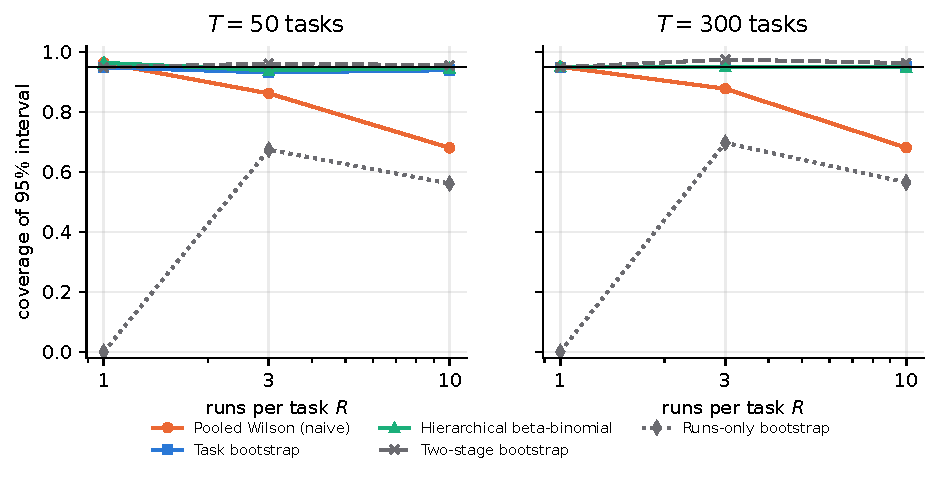
\includegraphics[width=\linewidth]{figures/coverage.pdf}
\caption{Coverage of nominal 95\% intervals for the benchmark score as runs per task grow (task sd $1.5$, interaction sd $0.5$, true score $\approx 0.43$). Pooling all runs breaks down already at three runs.}\label{fig:coverage}
\end{figure}

\paragraph{Robustness of coverage (E3).} The ranking of methods holds across prevalence and task heterogeneity, but the task bootstrap is not uniformly near nominal (Figure~\ref{fig:covrob}). For $T\ge50$ and $R>1$ it covers \covrobBootMin{}--\covrobBootMax{} and the beta-binomial interval \covrobBBMin{}--\covrobBBMax{}. With $T=20$, one run per task and extreme prevalence with homogeneous tasks the percentile bootstrap covers only \covrobBootSmallMin{}--\covrobBootSmallMax{} (BCa: from \covrobBCaSmallMin{}) because the resampled score is nearly degenerate; the pooled Wilson interval is exact there and should be preferred. The runs-only bootstrap has zero coverage at $R=1$ (\covrobRunsOnlyOne{}) because it sees no variation. The pooled Wilson interval fails only when runs are clustered \emph{and} tasks differ: at ten runs and task sd $1.5$ it covers \covrobWilsonMin{}--\covrobWilsonMax{}, and it is roughly nominal when tasks are nearly homogeneous. Our recommendation is therefore conditional: task-level intervals when $R>1$ or $T\ge50$, and an exact binomial interval for very small single-run evaluations.
\begin{figure}[t]
\centering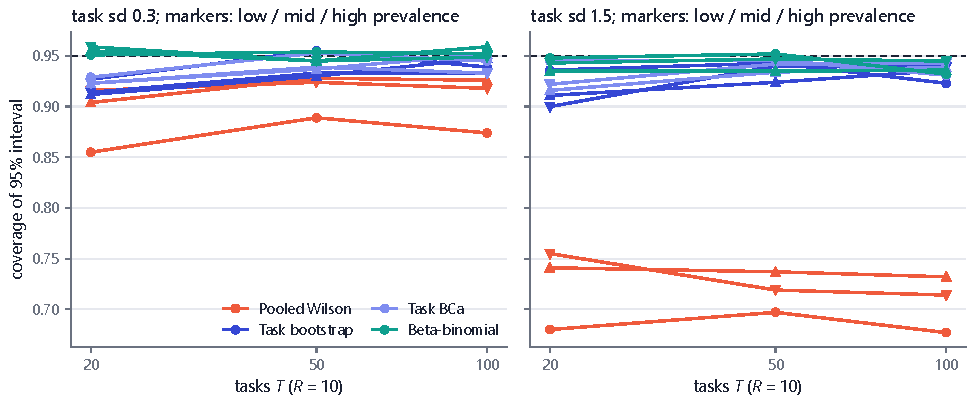
\includegraphics[width=\linewidth]{figures/coverage_robustness.pdf}
\caption{Coverage at ten runs per task for two task-heterogeneity levels and three prevalences (marker shape). Pooled Wilson loses coverage when tasks differ; the task-level methods approach the nominal level as $T$ grows.}\label{fig:covrob}
\end{figure}

\paragraph{Error rates of paired tests (RQ1).} With agent-by-task interaction sd $=1$, $T=100$ and ten runs per task, tests that treat each run as an independent pair reject a true null in \typeIPoolZ{} (two-proportion $z$-test) and \typeIPoolMc{} (run-level McNemar) of simulations, whereas the task-level sign-flip and bootstrap tests reject in \typeIPerm{} and \typeIBoot{} (Figure~\ref{fig:typeI}). With smaller interaction (sd $0.5$) run-level McNemar is still liberal (\typeIPoolMcLow). The pooled $z$-test is not always anti-conservative (it ignores pairing and is conservative at small $R$), so the harm of pooling is a loss of validity rather than a uniform inflation. Across all cells with a true null the sign-flip test rejects between \typeIPermMin{} and \typeIPermMax{}.
\begin{figure}[t]
\centering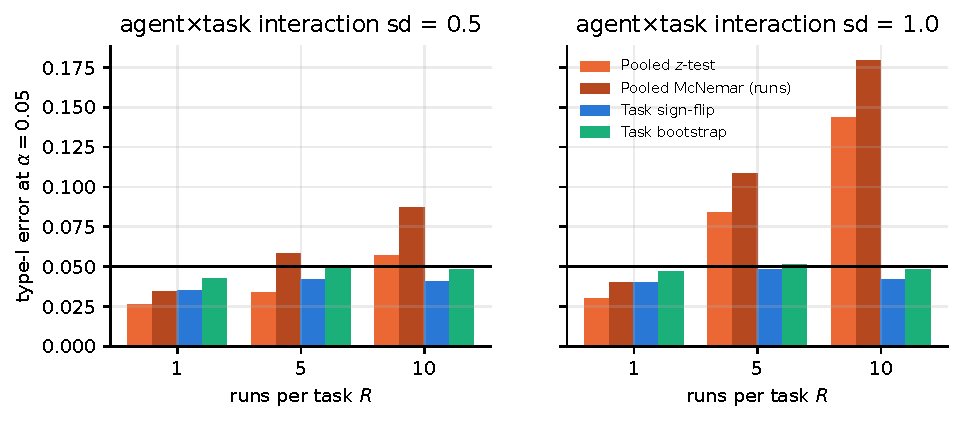
\includegraphics[width=\linewidth]{figures/typeI.pdf}
\caption{Type-I error at $\alpha=0.05$ for $T=100$ tasks and two agents of equal skill.}\label{fig:typeI}
\end{figure}

\paragraph{Weak null with skewed differences (E1).} The simulation above has symmetric per-task differences, where the sign-flip test is exact. We also generated paired differences with mean zero but heavy skewness (a rare large win offset by frequent small losses; skewness up to $5.5$). No procedure exceeded the pre-specified tolerance of 2 points over 5\% at $T\ge100$ (Figure~\ref{fig:asym}): across all cells the largest rejection rates were \asymMaxSF{} for the sign-flip test, \asymMaxSSF{} for its studentised version, \asymMaxBoot{} for the paired bootstrap and \asymMaxT{} for the paired $t$-test, with Monte Carlo error of about 0.6 points. The sign-flip tests are conservative on average (mean rejection \asymMeanSF{}); the bootstrap and $t$ tests are on average at nominal (\asymMeanBoot{}) but occasionally 1--2 points above it. We therefore keep the sign-flip test as the default, but we state its exactness only for symmetric differences.
\begin{figure}[t]
\centering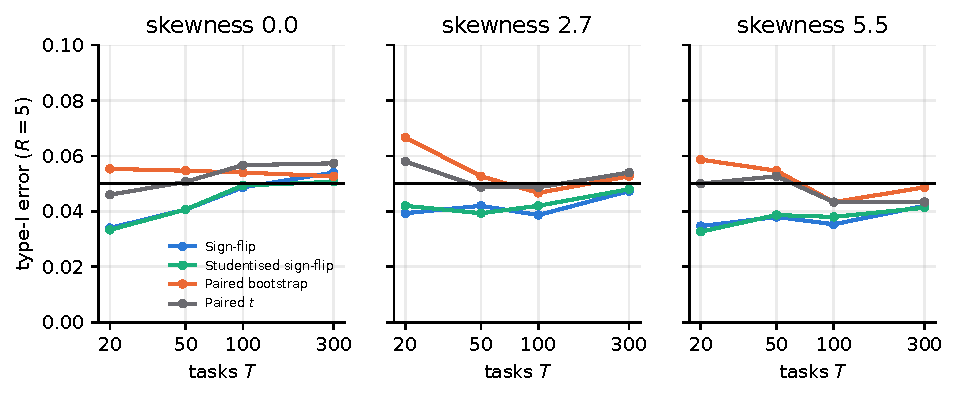
\includegraphics[width=\linewidth]{figures/asymmetric_null.pdf}
\caption{Type-I error at $\alpha=0.05$ with $R=5$ for paired differences with mean zero and increasing skewness (left to right).}\label{fig:asym}
\end{figure}

\paragraph{Tasks or repeats? (RQ2, E2).} In the original configuration (task sd $1.5$, interaction sd $0.6$) the standard error of the score difference at a fixed budget of \designBudget{} runs grows by a factor of \designSEratio{} between one and twenty runs per task, and power falls from \designPowerOne{} to \designPowerTen{} (ten runs) and \designPowerTwenty{} (twenty runs) (Figure~\ref{fig:design}); the analytic variance model predicts the simulated standard errors to within \designMaxSEgap{}. This is not a general law. Across nine configurations (E2, Figure~\ref{fig:alloc}) the standard-error ratio of ten versus one run per task is \allocRatioLow{} when the interaction sd is $0.2$ (repeats cost nothing) and \allocRatioHigh{} when it is $1.0$; the task standard deviation hardly matters, because the task main effect cancels in a paired difference. The cost-optimal number of runs per task for a task that costs ten runs is \allocRstarTenLow{} with small interaction and \allocRstarTenHigh{} with large interaction. If the pool of tasks is capped (for example at 120), the question changes and the extra budget must go to repeats. Analytic and simulated standard errors agree to within \allocMaxSEgap{} in E2. Repeats are not useless: they identify run noise and enable pass$^k$.
\begin{figure}[t]
\centering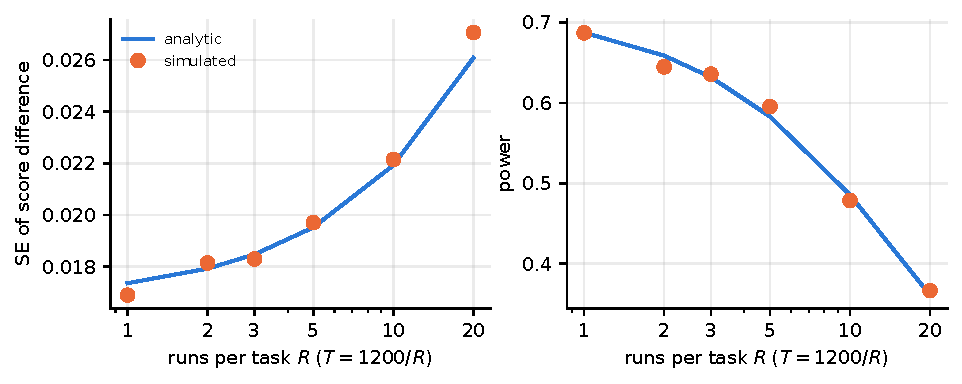
\includegraphics[width=\linewidth]{figures/design.pdf}
\caption{Fixed budget $B=1200$ runs, $T=B/R$ tasks. Left: standard error of the difference between two agents; right: power of the paired $t$-test.}\label{fig:design}
\end{figure}
\begin{figure}[t]
\centering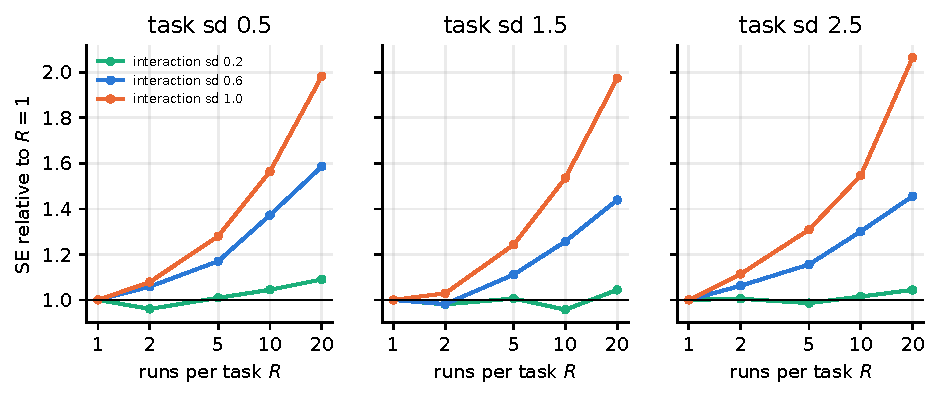
\includegraphics[width=\linewidth]{figures/allocation.pdf}
\caption{Standard error of the score difference at fixed budget relative to one run per task, for three task heterogeneities and three interaction levels. Curves are flat when the interaction is small.}\label{fig:alloc}
\end{figure}

\paragraph{Sequential evaluation (RQ4).} Applying a fixed-sample test after every task (``peeking'') and stopping at the first $p<0.05$ gives \seqNullPeek{} false positives under the null, against \seqNullSeq{} for the confidence sequence and \seqNullFixed{} for the fixed-$n$ test (Figure~\ref{fig:seq}). The price is power: with a true difference of \seqMidDiff{} points the sequence decides in \seqPowerSeqMid{} of runs against \seqPowerFixedMid{} for the fixed-$n$ test at the full budget of \seqBudget{} tasks. When the effect is large it stops early (median \seqLargeMedianTasks{} tasks for the largest difference). Confidence sequences buy the right to stop at any time; they do not make evaluation cheaper at a given power.
\begin{figure}[t]
\centering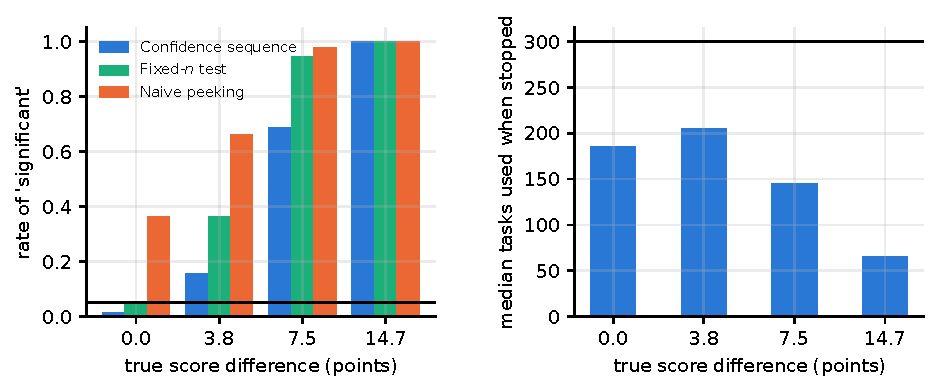
\includegraphics[width=\linewidth]{figures/sequential.pdf}
\caption{Sequential comparison, $R=3$ runs per task. Left: fraction declared significant (the line marks 5\%). Right: median number of tasks used when the sequence stops.}\label{fig:seq}
\end{figure}
Equivalence is only possible with a margin (E5, \seqmReps{} replications per cell). With margin zero ``equivalent'' was never declared (\seqmZeroMarginEquiv) and, for two agents of identical skill, the sequence stayed undecided in \seqmUndecidedTie{} of runs within 300 tasks: absence of a decision is not equivalence. With a margin of 10 points and a true gap of zero, equivalence was declared in \seqmEquivTrueTie{} of runs (median \seqmEquivTrueTieTasks{} tasks). When the true gap exceeded the margin, equivalence was declared in at most \seqmFalseEquivMax{} of runs, below $\alpha$, as the theory requires. Narrow margins are rarely reachable with 300 tasks.

\paragraph{Ranking uncertainty and near ties (RQ3, E6).} Bootstrap rank intervals are conservative for the population ranking (coverage \rankCovMin--\rankCovMax{} for nominal 95\%), and $P(\mathrm{best})$ is reasonably calibrated, noisily at $T=50$ (Figure~\ref{fig:rankcal}). In a six-agent leaderboard with one exactly tied pair and one pair \rankpwCloseTrue{} points apart, Holm-adjusted tests rejected the tied pair in at most \rankpwFWE{} of replications in every cell (the family-wise error is controlled and the procedure is conservative), but separated the close pair in only \rankpwCloseRej{} of replications even with 500 tasks and three runs per task (and \rankpwCloseRejSmall{} with 50 tasks). Small gaps are, in practice, not resolved by realistic benchmark sizes.
\begin{figure}[t]
\centering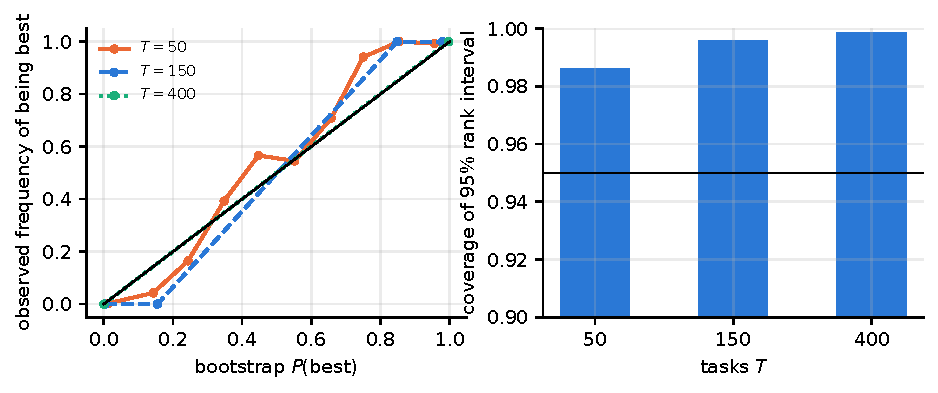
\includegraphics[width=\linewidth]{figures/ranking_calibration.pdf}
\caption{Six agents of known skill. Left: calibration of bootstrap $P(\mathrm{best})$. Right: coverage of the 95\% rank interval.}\label{fig:rankcal}
\end{figure}

\subsection{Re-analysis of public results (RQ3)}\label{sec:public}
\paragraph{SWE-bench Verified.} The \sweNAgents{} entries yield \sweNPairs{} agent pairs. After Holm adjustment \sweFracHolm{} are distinguishable at $\alpha=0.05$ (\sweFracBH{} with Benjamini--Hochberg; \sweFracRaw{} without correction), so \sweIndistHolm{} cannot be separated; ``cannot be separated'' means not detected, not equal. The result is driven by the score gap (Figure~\ref{fig:swe}): pairs 2--5 points apart are separable in \sweGapSmallHolm{} of cases after correction, pairs 5--10 points apart in \sweGapMidHolm{}, and larger gaps almost always. The smallest distinguishable gap is \sweMinGap{} points and the median is \sweMedGap. The top entry (\sweTopScore) has a 95\% rank interval of 1--\sweTopRankHi{} and probability \sweTopPBest{} of being best.
\begin{figure}[t]
\centering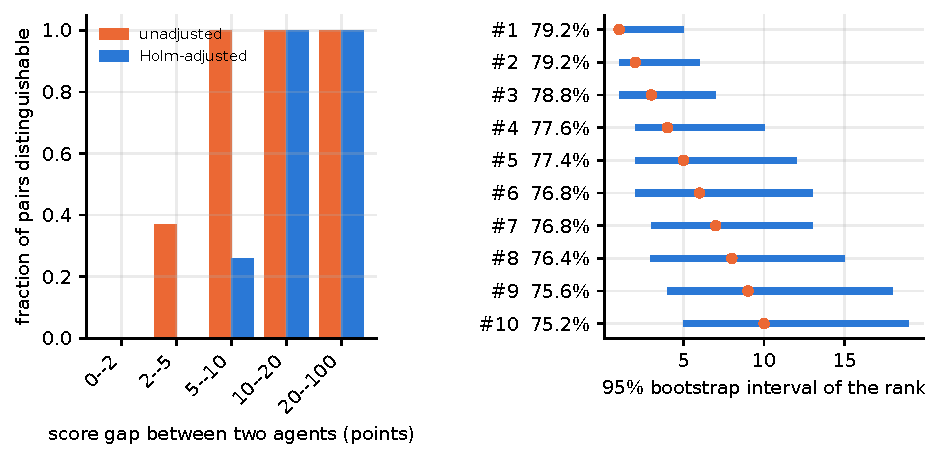
\includegraphics[width=\linewidth]{figures/swebench.pdf}
\caption{SWE-bench Verified, \sweNAgents{} public entries. Left: fraction of pairs distinguishable by score gap. Right: top-10 scores with 95\% bootstrap rank intervals.}\label{fig:swe}
\end{figure}

\paragraph{Sensitivity to undocumented evaluation details.} The headline count of adjacent positions depends on the entries retained (Table~\ref{tab:swerobust}). Among all entries, \sweAllAdjHolm{} of adjacent leaderboard positions are distinguishable after Holm over \emph{all} pairs (\sweAllAdjRaw{} without correction). Restricting to entries whose coverage of the 500 instances could be verified gives \sweCovAdjHolm{}; restricting to entries that declare a single attempt (\sweNSingle{} entries) gives \sweSingleAdjHolm{}, because with fewer, more spread-out entries adjacent gaps are larger. The share of separable pairs is stable (\sweCovFracHolm{} coverage-verified, \sweSingleFracHolm{} single-attempt, \sweBothFracHolm{} both). The qualitative conclusions, that most pairs but almost no adjacent positions are separable, therefore hold across the subsets, whereas the earlier claim that \emph{none} of the adjacent positions is distinguishable is not robust: it is true only for the full set. Many entries are best-of-$n$ or multi-sample systems and different scaffolds, budgets and dates are mixed; the comparison is of leaderboard rows, not of models.
\begin{table}[t]
\centering\small
\caption{SWE-bench Verified sensitivity analysis. ``Adjacent'' counts distinguishable neighbouring leaderboard positions; Holm is applied over all pairs of the subset.}\label{tab:swerobust}
\begin{tabular}{lrrrr}
\toprule
Subset & Entries & Pairs separable (\%) & Adjacent, Holm & Adjacent, unadjusted \\
\midrule
All entries & 129 & 71.7 & 0/128 & 2/128 \\
Coverage verified & 110 & 71.7 & 1/109 & 3/109 \\
One attempt declared & 41 & 69.3 & 3/40 & 6/40 \\
Both & 37 & 68.5 & 2/36 & 5/36 \\
\bottomrule
\end{tabular}

\end{table}

\paragraph{$\tau$-bench.} For gpt-4o versus Claude 3.5 Sonnet with four trials per task, the retail gap is \tauRetailDiff{} points (95\% task-bootstrap interval \tauRetailCI), task-level sign-flip $p=\tauRetailPPerm$ ($p=\tauRetailPHolm$ after Holm adjustment over the two domains); the pooled-runs $z$-test gives $p=\tauRetailPPool$. The task-level exact McNemar test on per-task majority outcomes, which discards run-level information, gives $p=\tauRetailPTaskMc$, so the retail result is not independent of the choice of test. In airline the gap is \tauAirlineDiff{} points \tauAirlineCI{} with $p=\tauAirlinePPerm$ (pooled $p=\tauAirlinePPool$): not detected with \tauAirlineTasks{} tasks, which does not show that the two models are equal. Plug-in power calculations suggest about \tauAirlineNeed{} tasks would be needed at the observed airline gap (retail: \tauRetailNeed{}), but these figures are very uncertain: a task bootstrap of the pilot gives 95\% intervals of \tauAirlineNeedLo{}--\tauAirlineNeedHi{} (airline) and \tauRetailNeedLo{}--\tauRetailNeedHi{} (retail) tasks. Variance is dominated by run noise (\tauAirlineRunShare{} airline, \tauRetailRunShare{} retail) and task difficulty (\tauAirlineTaskShare, \tauRetailTaskShare), with agent-by-task interaction of \tauAirlineInterShare{} and \tauRetailInterShare. Figure~\ref{fig:tau} contrasts pass@$k$ with pass$^k$: both models look strong when one success in $k$ suffices and much weaker when all $k$ must succeed. The data cover two models and two domains, and the model versions are those of the released trajectories.
\begin{figure}[t]
\centering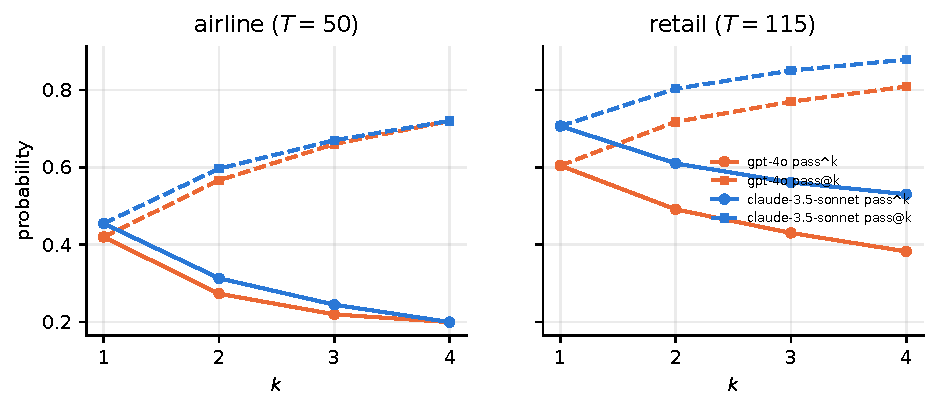
\includegraphics[width=\linewidth]{figures/taubench.pdf}
\caption{$\tau$-bench, four trials per task: pass$^k$ (solid) falls and pass@$k$ (dashed) rises with $k$.}\label{fig:tau}
\end{figure}

\IfFileExists{sections/real.tex}{\subsection{Local open-weight models (RQ5)}\label{sec:real}
\paragraph{Setup and headline numbers.} \realNModels{} models, \realNTasks{} tasks, \realNRuns{} runs each (\realNAttempts{} runs in total). Success rates range from \realWorstScore{} (\realWorstModel) to \realBestScore{} (\realBestModel); the full table with pass$^k$ and per-family scores is in Appendix~\ref{app:real}. Figure~\ref{fig:real} (left) shows 95\% task-bootstrap intervals. Scores here combine two things: protocol validity (does the model emit a parseable action in the uniform text protocol?) and task competence. The quantised variant \texttt{qwen2.5-3b-q2} never produced a parseable action (\realFloorNoAction{} of its runs end with no tool call), so its score of zero measures protocol failure and says nothing about the underlying agent; we keep it as a degenerate control rather than dropping it silently, and it contributes to the variance decomposition and the pair counts as a floor. Without it, \realNIndistNoQtwo{} of the \realNPairsNoQtwo{} remaining pairs are not separable after Holm (recomputed from the stored pairwise $p$-values); the variance decomposition and the rankings without it could not be recomputed because the per-run outcomes are not stored (Appendix~\ref{app:repro}). Backend errors (\realBackendErr{} runs, \realBackendErrShare{}) are scored as failures. Results are specific to this protocol and these quantised models.
\begin{figure}[t]
\centering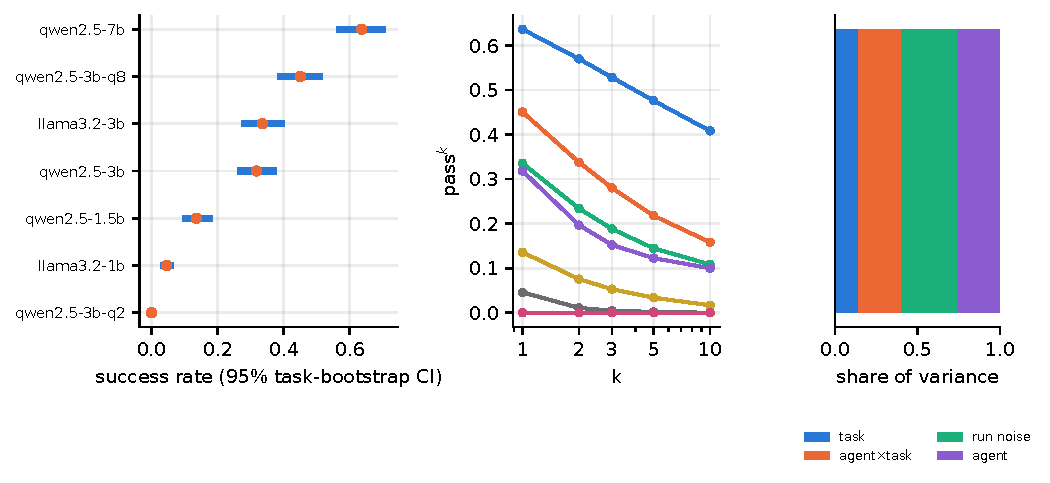
\includegraphics[width=\linewidth]{figures/real_main.pdf}
\caption{Local models on the \realNTasks-task core suite, \realNRuns{} runs per task. Left: success rate with 95\% task-bootstrap interval. Middle: pass$^k$. Right: variance decomposition of the full agents-by-tasks-by-runs array.}\label{fig:real}
\end{figure}

\paragraph{Reliability is much lower than the headline score.} The best model's score of \realBestScore{} falls to \realBestPassThree{} for pass$^3$ and \realBestPassTen{} for pass$^{10}$: a model that solves a task on average does not solve it every time. Run noise accounts for \realRunShare{} of the variance of single runs, task difficulty for \realTaskShare, agent-by-task interaction for \realInterShare{} and agent identity for \realModelShare. The agent share describes the spread of these seven fixed models, not a population variance. Run noise is of the same order as the quantity of interest, so a one-run evaluation is a noisy measurement even here.

\paragraph{Ranking: the hypothesis is only partly borne out.} Because the models differ a lot in capability, the ranking is well determined: \realNIndist{} of \realNPairs{} pairs are not separable after Holm correction (\realClosestA{} versus \realClosestB{}, a gap of \realClosestDiff{} points, adjusted $p=\realClosestP$), and the split-half rank correlation is \realSplitTau. This contrasts with SWE-bench, where scores are close; the statistical problems are most severe when systems are close, not absent otherwise. A plug-in power calculation says that resolving a 5-point difference between two of these agents at 80\% power needs about \realTasksNeeded{} tasks at ten runs per task, more than three times the suite size, and the minimum detectable difference of the current design is \realMDE{} points; both are estimates from one pilot and carry the uncertainty documented for $\tau$-bench above. With the cost model of Section~\ref{sec:power}, the optimal number of runs per task is \realOptRuns{} when a task costs as much as ten runs.

\subsection{Ablations on real data}\label{sec:ablation}
\paragraph{Tasks versus runs.} The sub-designs are random subsets of the same \realNTasks{} tasks and ten runs, compared with the ranking and the significant pairs of the full data. The full-data ranking shares observations with every subsample and is itself an estimate, so this measures \emph{internal stability relative to the full observed sample}, not recovery of an independently known population ranking; the pairs that are significant in the full data are also selected by the same data, so sign agreement among them is optimistic. Recovery of a known ranking is examined in the simulation (E6, Figure~\ref{fig:rankcal}); a split-sample analysis on independent halves would require the per-run outcomes, which are not stored. Sub-sampling the real data (Figure~\ref{fig:realabl}), a ranking from all \realNTasks{} tasks with one run per task has Kendall $\tau=\ablTauOneRun$ with the full-data ranking and separates \ablFracOneRun{} of the pairs, against \ablFracAllRuns{} with ten runs. With only \ablFewTasks{} tasks and one run the ranking correlation is $\tau=\ablTauFewTasks$ and only \ablFracFewTasks{} of pairs are separated. Since the large gaps are easy, rank correlation saturates quickly; the number of \emph{separated pairs} is the informative measure and it keeps growing with both tasks and runs. We did not repeat the fixed-budget comparison of Section~\ref{sec:sim} on real data, so the simulation result on tasks versus runs is neither confirmed nor refuted here.
\begin{figure}[t]
\centering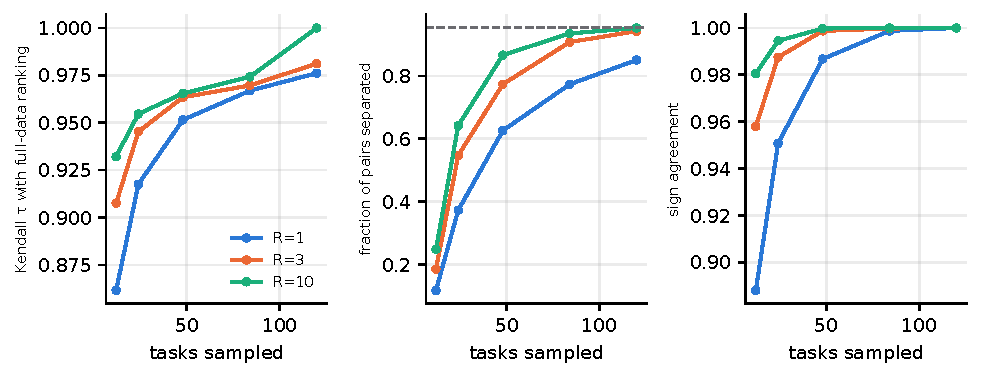
\includegraphics[width=\linewidth]{figures/real_ablation.pdf}
\caption{Sub-designs of the real data (random subsets of tasks and runs, 200 draws). Left: Kendall $\tau$ with the full-data ranking. Middle: fraction of the \realNPairs{} pairs separated (paired $t$-test, Holm); the dashed line is the full data. Right: sign agreement for pairs that are significant in the full data. The reference is the full-data result, which shares observations with every subsample, so all panels measure stability relative to the observed sample, not accuracy against a known truth.}\label{fig:realabl}
\end{figure}

\paragraph{Sequential stopping.} Applying the confidence sequence to tasks in random order, \seqRealDecided{} of the \seqRealNSig{} pairs that are significant on the full data are decided before the tasks run out, with a median of \seqRealMedTasks{} tasks. This re-orders existing results; it is not a live stopping experiment. Large gaps are settled after a few tens of tasks; close pairs are not decided within the suite, as in the simulation.

\paragraph{Cost profile.} Figure~\ref{fig:realprof} reports tokens and wall-clock per run. The weakest functioning model, \realMaxStepLimitModel, hits the step limit in \realMaxStepLimit{} of runs and consumes the most tokens: failure is not cheap, so cost per success varies more than cost per run. Wall-clock was measured with four parallel workers on one machine and is indicative only.
\begin{figure}[t]
\centering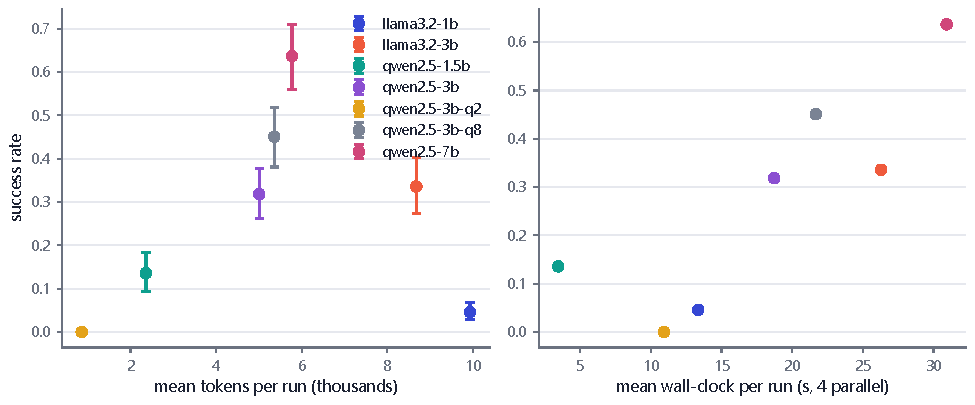
\includegraphics[width=\linewidth]{figures/real_profile.pdf}
\caption{Success rate against mean tokens (left) and wall-clock (right) per run.}\label{fig:realprof}
\end{figure}
}{}

\section{Discussion}
The simulation results are not surprising in isolation (clustered data need clustered inference), but their size is. Reporting a single pooled interval from several runs is common and, with ten runs per task, wrong by almost thirty coverage points. The public re-analysis shows that the consequence for leaderboards is concrete: with 500 instances and one run each, differences of up to about five points are routinely within noise, and the neighbours on the leaderboard are not separated. Neither finding says that leaderboards are useless: large gaps are reliably detected, and the top of the SWE-bench ranking is clearly above the bottom. They say that rank positions near each other should not be read as an ordering.

\paragraph{Recommendations.} (i) Treat tasks as the sampling unit; report task-bootstrap or hierarchical intervals. (ii) Compare agents on the same tasks with paired task-level tests and correct for multiplicity. (iii) Plan with the variance decomposition: more tasks before more repeats, unless reliability (pass$^k$) is the target or tasks are expensive relative to runs. (iv) Report pass$^k$ with pass@$k$. (v) If monitoring an evaluation as it runs, use a confidence sequence, not repeated fixed-sample tests. (vi) Publish per-task, per-run outcomes so that others can do this.

\paragraph{Refuted or weakened parts of the hypothesis.} \REALREFUTED
\section{Limitations, Ethics and Broader Impact}\label{sec:limits}
\paragraph{Limitations.} The local-model evaluation uses small quantised models on one machine, so absolute scores and failure modes do not transfer to frontier agents; generality rests on the simulations and the public re-analysis. The environments are cleaner than real software tasks and checkers verify only the state the generator anticipates. Tasks are i.i.d.\ draws from the population defined by our generator, so intervals refer to that population, not to ``ability''. The variance decomposition is linear on the probability scale. The SWE-bench re-analysis assumes full coverage of the 500 instances by every submission and ignores differences in scaffolds, budgets and submission dates; the tau-bench data cover two models. Confidence sequences are conservative. Task difficulty in the benchmark is controlled by knobs we chose and is not calibrated to any human notion of difficulty.
\paragraph{Ethics and impact.} No human subjects or personal data are involved; all environments are synthetic and all public data are used under their licenses (tau-bench: MIT; the SWE-bench experiments repository declares no license, so we store only derived aggregates and a download script). Better error bars can reduce overclaiming in agent evaluation, but statistical rigour can also be used to dismiss real improvements; a non-significant result is not evidence of equivalence, and we provide equivalence-margin stopping for that reason. All experiments used free, local, open-weight models and public data; no paid API was used.
\section{Conclusion}
Agent leaderboards carry less information than their precision suggests. A statistically principled treatment of tasks, runs and their interaction, tested against ground truth, shows where differences are real and tells practitioners how to spend an evaluation budget. We release the library, the benchmark, the playground and all scripts to regenerate every number in this paper.

\section{Limitations, Ethics and Broader Impact}\label{sec:limits}
\paragraph{Limitations.}
\emph{Inferential target.} Tasks are treated as i.i.d.\ draws from the population defined by our generator (or, for public data, from the benchmark), so intervals refer to that population and not to ``ability''; tasks within a benchmark are often related (same repository, same domain), which would make our task-level intervals optimistic. Agents are fixed effects.
\emph{Local models.} The evaluation uses small quantised models, one machine (an Apple laptop reported by the author; hardware is not verifiable from the stored results), one prompt protocol, temperature 0.7 and no fault injection, so absolute scores and failure modes do not transfer to frontier agents. Raw trajectories and caches are not retained; the stored aggregates cannot be re-derived from raw runs.
\emph{Benchmark.} The environments are cleaner than real software tasks; checkers verify only the state the generator anticipates; difficulty knobs are not calibrated to any human notion of difficulty.
\emph{Statistics.} The variance decomposition is linear on the probability scale; the simulation model is one generator whose robustness we explored only along the axes listed in Section~\ref{sec:protocol}; confidence sequences require i.i.d.\ tasks and are conservative; plug-in power and tasks-needed figures are highly uncertain; Monte Carlo errors are 0.6--0.7 points.
\emph{Public data.} The SWE-bench files do not state coverage or attempts; we audit them but \sweNUnverif{} entries have no public logs. Scaffolds, budgets and dates are mixed. The $\tau$-bench data cover two models and two domains.
\paragraph{Ethics and impact.} No human subjects or personal data are involved; environments are synthetic and public data are used under their licenses ($\tau$-bench: MIT; the SWE-bench experiments repository declares no license, so we store only derived aggregates and a download script). Better error bars can reduce overclaiming, but rigour can also be used to dismiss real improvements; a non-significant result is not evidence of equivalence, which is why equivalence requires a margin. All experiments used free, local, open-weight models and public data; no paid API was used.

\section{Conclusion}
Agent leaderboards carry less information than their precision suggests, most of all for close systems. Treating the task as the sampling unit, testing the procedures against ground truth including where they fail, and auditing what public data do and do not document give a more defensible reading of agent results. We release the library, the benchmark, the scripts and the stored results so that every number in this paper can be regenerated from \texttt{results/}.


\bibliography{references}
\bibliographystyle{tmlr}

\appendix
\section{Mathematical details}\label{app:ems}
For balanced data with $M$ agents, $T$ tasks and $R$ runs, the expected mean squares of the crossed model are
\begin{align*}
E[MS_m]&=\sigma^2_e+R\sigma^2_{mt}+TR\sigma^2_m, & E[MS_t]&=\sigma^2_e+R\sigma^2_{mt}+MR\sigma^2_t,\\
E[MS_{mt}]&=\sigma^2_e+R\sigma^2_{mt}, & E[MS_e]&=\sigma^2_e,
\end{align*}
and the estimators solve these for the components, truncating negative values at zero (the raw values are retained). With $R=1$ the interaction and error are confounded; the library flags this. For one agent, the one-way model gives $\hat\sigma^2_t=(MS_b-MS_w)/R$ and $\hat\sigma^2_e=MS_w$, which equals the REML estimate for balanced data (verified against statsmodels in the test suite).

\paragraph{Unbiasedness of pass$^k$.} If $C\sim\mathrm{Bin}(n,p)$ then $E\binom{C}{k}=\binom{n}{k}p^k$, so $\binom{C}{k}/\binom{n}{k}$ is unbiased for $p^k$; similarly $E\binom{n-C}{k}=\binom{n}{k}(1-p)^k$.

\paragraph{Pooled design effect.} Writing $\bar Y=\frac1T\sum_t \hat p_t$ with $\hat p_t\mid p_t\sim\mathrm{Bin}(R,p_t)/R$, the law of total variance gives $\mathrm{Var}(\bar Y)=\tau^2/T+E[p_t(1-p_t)]/(TR)$ and $E[p_t(1-p_t)]=p(1-p)-\tau^2$.

\paragraph{Optimal runs.} Minimising $(s_t+s_e/R)(c_\text{task}+Rc_\text{run})$ over $R>0$ gives $R^\star=\sqrt{s_ec_\text{task}/(s_tc_\text{run})}$; the planner evaluates the two neighbouring integers.

\section{Tool-protocol defect observed in Ollama}\label{app:ollama}
With Ollama 0.40.8 (macOS, Apple silicon), the native \texttt{/api/chat} tool-calling interface returned an empty message (no content, no tool calls) for \texttt{qwen2.5:3b} on a file-creation task when eight tools were declared, although the raw generation obtained from the \texttt{/api/generate} endpoint with the model's own template contained a well-formed \texttt{<tool\_call>} block. The failure was deterministic across seeds and temperatures; it disappeared with a single declared tool or without a system message. Because of this, all experiments use the uniform text protocol of Section~\ref{sec:bench}. The observation is about one server version, not about the model.

\section{Prompts}\label{app:prompts}
\paragraph{System prompt.}
{\small\verbatiminput{generated/system_prompt.txt}}
\paragraph{Tool section appended to the system prompt.}
{\small\verbatiminput{generated/tools_prompt.txt}}

\section{Full coverage table}\label{app:tables}
\begin{table}[h]
\centering\small
\caption{Coverage (\%) of nominal 95\% intervals for the benchmark score; wilson, CP: pooled binomial intervals; the rest respect the task structure. $T$: tasks, $R$: runs per task.}
20 & 1 & 94.9 & 94.9 & 91.2 & 94.0 & 91.2 & 94.9 \\
20 & 3 & 87.9 & 89.6 & 93.3 & 94.7 & 96.5 & 95.0 \\
20 & 10 & 68.2 & 70.2 & 92.5 & 94.2 & 95.2 & 93.8 \\
50 & 1 & 96.4 & 96.4 & 94.9 & 96.2 & 94.9 & 96.4 \\
50 & 3 & 86.2 & 87.9 & 93.2 & 93.6 & 96.2 & 93.9 \\
50 & 10 & 68.0 & 69.2 & 94.0 & 94.5 & 95.6 & 94.7 \\
100 & 1 & 94.4 & 96.0 & 94.3 & 94.8 & 94.3 & 94.4 \\
100 & 3 & 88.5 & 88.5 & 94.9 & 95.1 & 96.8 & 95.0 \\
100 & 10 & 68.3 & 68.3 & 94.8 & 94.8 & 96.4 & 95.1 \\
300 & 1 & 95.1 & 95.1 & 94.9 & 95.2 & 94.9 & 95.1 \\
300 & 3 & 87.8 & 88.9 & 95.1 & 95.2 & 97.5 & 95.2 \\
300 & 10 & 68.1 & 68.8 & 95.0 & 95.0 & 96.3 & 94.9 \\

\end{table}
\IfFileExists{generated/tab_appendix_real.tex}{\begin{tabular}{lrrrrrrrrrrr}
\toprule
Model & score & pass$^3$ & pass$^{10}$ & steps & step-limit & fs & sql & crm & booking & forms & tabular \\
\midrule
qwen2.5-7b & 63.7 & 52.9 & 40.8 & 6.0 & 2\% & 90 & 57 & 55 & 88 & 63 & 28 \\
qwen2.5-3b-q8 & 45.1 & 28.0 & 15.8 & 4.7 & 1\% & 64 & 62 & 60 & 64 & 15 & 4 \\
llama3.2-3b & 33.6 & 18.8 & 10.8 & 8.5 & 22\% & 26 & 24 & 30 & 74 & 39 & 8 \\
qwen2.5-3b & 31.8 & 15.2 & 10.0 & 4.8 & 6\% & 56 & 25 & 36 & 52 & 12 & 10 \\
qwen2.5-1.5b & 13.6 & 5.3 & 1.7 & 2.9 & 0\% & 28 & 12 & 3 & 34 & 3 & 0 \\
llama3.2-1b & 4.6 & 0.5 & 0.0 & 8.5 & 42\% & 4 & 8 & 0 & 14 & 2 & 0 \\
qwen2.5-3b-q2 & 0.0 & 0.0 & 0.0 & 1.0 & 0\% & 0 & 0 & 0 & 0 & 0 & 0 \\
\bottomrule
\end{tabular}
}{}

\section{Reproducibility checklist}
\begin{itemize}
\item Code, benchmark generator, configs and all scripts: \url{https://github.com/fragompul/agentaudit}; \texttt{make reproduce} regenerates simulation results, re-analyses and figures; every number in this paper is produced by \texttt{scripts/make\_paper\_assets.py} from \texttt{results/}.
\item Seeds are fixed in every script; model tags and quantisations are in \texttt{configs/models.json}; the test suite runs without network access (coverage above 90\%, \texttt{mypy --strict}).
\item Raw trajectories and the record/replay caches are released as release assets (they are not stored in git).
\item Compute: a single Apple M5 laptop with 16\,GB unified memory; no cloud, no paid API.
\end{itemize}

\end{document}
